\subsection{Эксперимент 2. Анализ оптимальных  параметров для SGD.}
\subsubsection{Дизайн эксперимента}
В ходе данного эксперимента исследовались параметры для SGD. Дизайн эксперимента полностью повторяет предыдущий эксперимент за исключением того факта, что к параметрам из предыдущего эксперимента добавился размер батча  ({\itshape batch\_size}). 
\subsubsection{Результаты эксперимента}
Сразу же заметим, что зависимость графиков от времени и от эпох очень похожи, поэтому все графики будут находиться в  {\bfseries Приложении Б}, а здесь же используются только необходимые.
\begin{enumerate}
	\item {\bfseries  Выбор $\alpha$}
	
	Фиксируем $\beta = 1$, $\omega_0 = 0 \in \mathbb{R}^D$, $batch\_size=10000$ и по логарифмической сетке рассмотрим различные параметры $\alpha$ (см. рис.\ref{eq:exp2_fig1}):
    %\newsavebox{\myimage}
    \begin{figure*}[h]
        \begin{subfigure}{.5\textwidth}
            \centering
            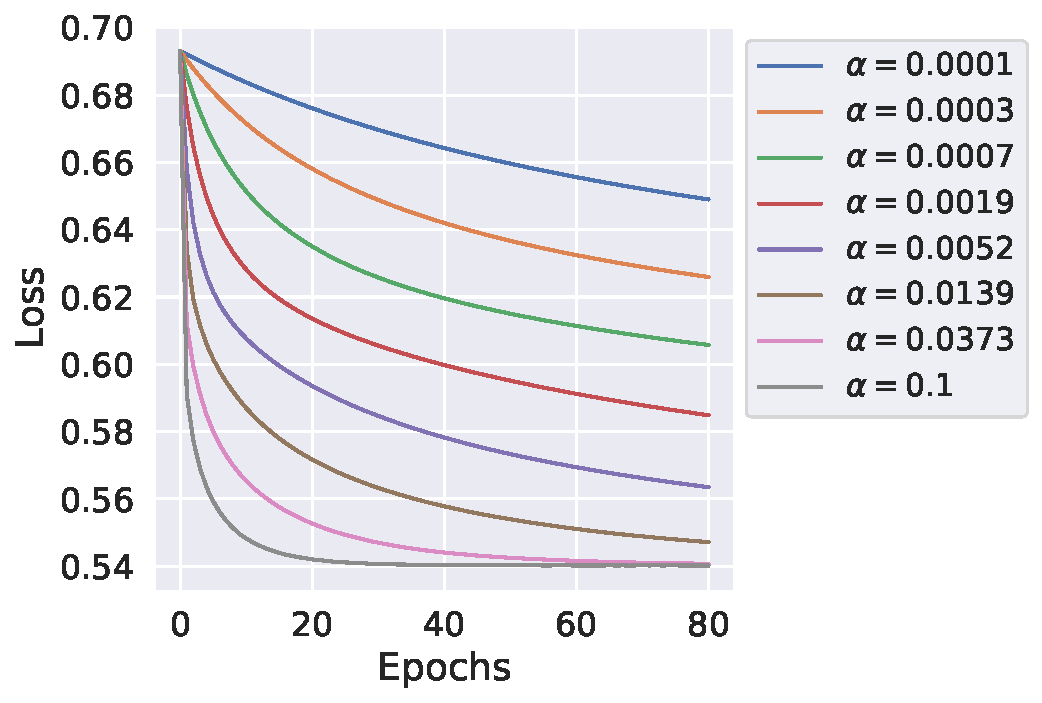
\includegraphics[width=\linewidth]{./experiment2/alpha/sgd_loss__iters.pdf}
            \caption{}
        \end{subfigure}%
        \begin{subfigure}{.5\textwidth}
            \centering
            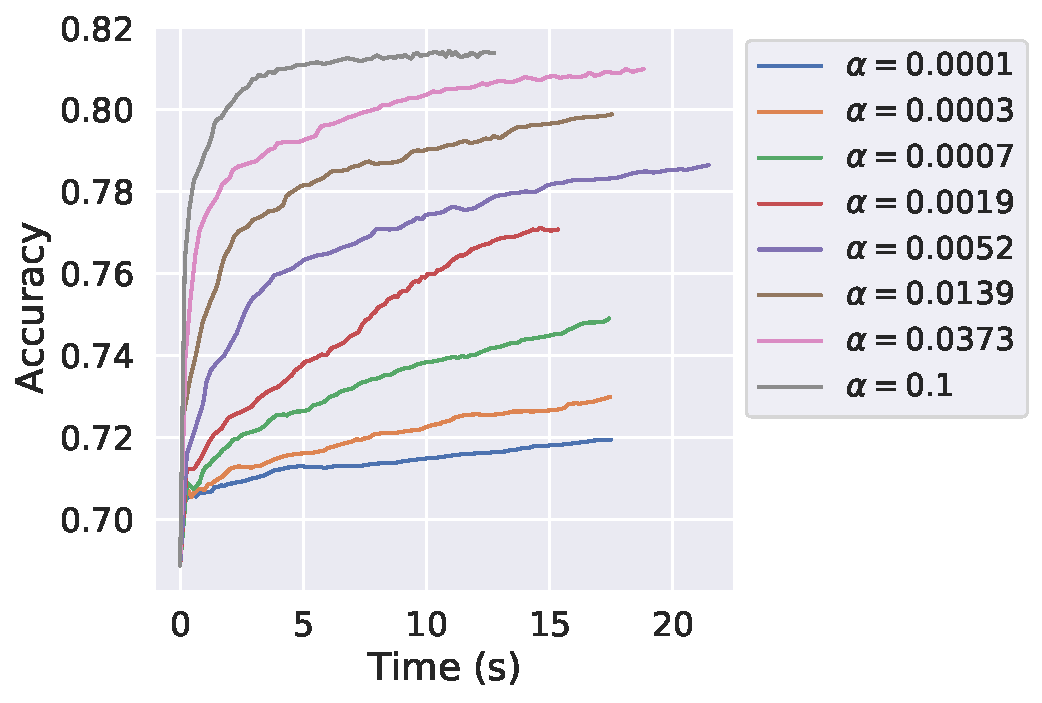
\includegraphics[width=\linewidth]{./experiment2/alpha/sgd_acc_time.pdf}
            \caption{}
        \end{subfigure}
    \caption{}\label{eq:exp2_fig1}
	\end{figure*}
	Из графика (см. рис.\ref{eq:exp2_fig1}) следуют точно такие же выводы как и в случае градиентного спуска, то есть при увеличении $\alpha$ (не больше~1) функция потерь быстрее стремиться к минимуму. При больших $\alpha$ уже видна осцилляция, а при дальнейшем увеличении задача минимизации уже не разрешима (см. {\bfseries Приложение Б}).

	Посмотрим на accuracy. Как видно из рис. \ref{eq:exp2_fig1} на валидационной выборке точность наилучшая при $\alpha=0.1$, при этом время работы при различных значениях данного параметра почти одинаково

	\item {\bfseries  Выбор $\beta$}
	
	Фиксируем $\alpha = 0.1$, $\omega_0 = 0 \in \mathbb{R}^D$, $batch\_size=10000$ и по логарифмической сетке рассмотрим различные параметры $\beta$ (см. рис.\ref{eq:exp2_fig2}):
	%\newsavebox{\myimage}
    \begin{figure*}[h]
        \begin{subfigure}{.5\textwidth}
            \centering
            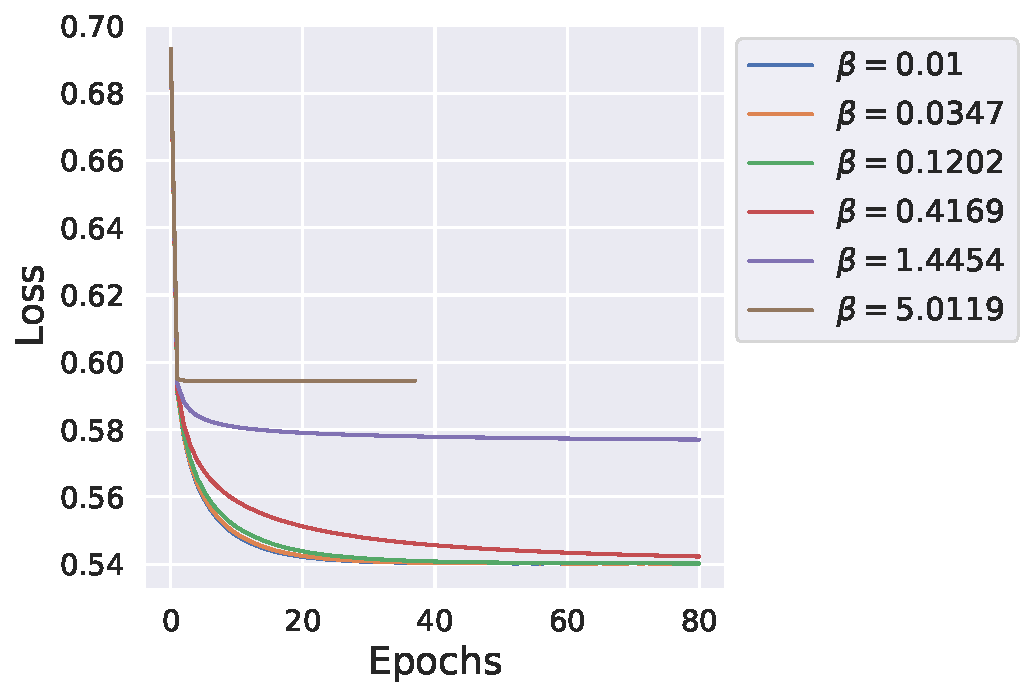
\includegraphics[width=\linewidth]{./experiment2/beta/sgd_loss__iters.pdf}
            \caption{}
        \end{subfigure}%
        \begin{subfigure}{.5\textwidth}
            \centering
            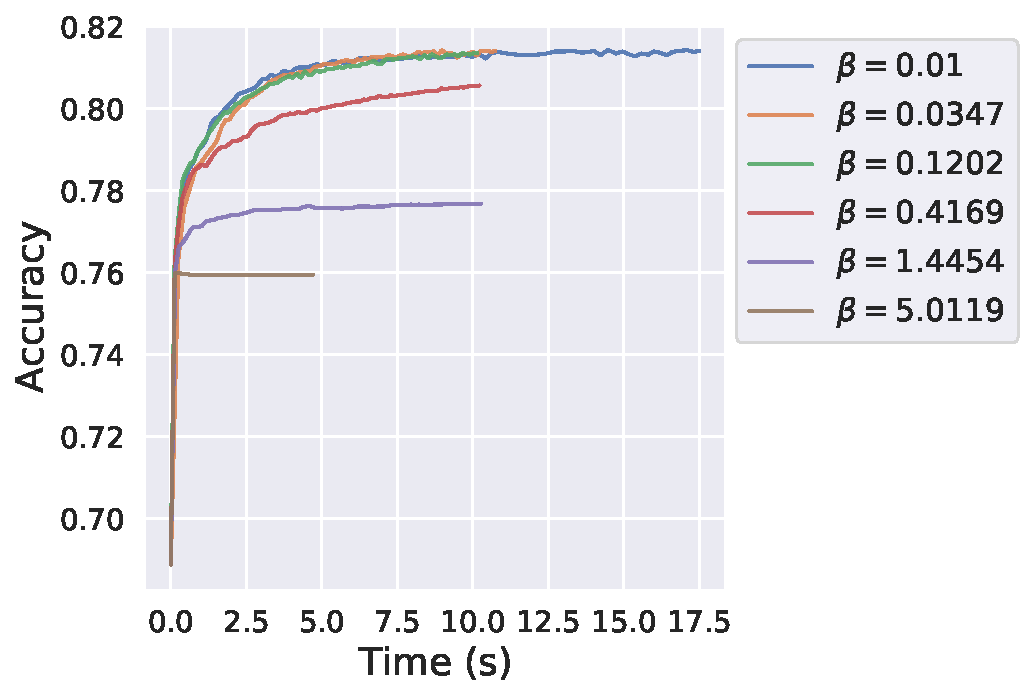
\includegraphics[width=\linewidth]{./experiment2/beta/sgd_acc_time.pdf}
            \caption{}
        \end{subfigure}
    \caption{}\label{eq:exp2_fig2}
    \end{figure*}
	Видно (см. рис.\ref{eq:exp2_fig2}), что тут такая же зависимость как и в случае градиентного спуска, то есть при уменьшении $\beta$ функция потерь быстрее стремиться к минимуму. При больших $\beta$ быстро выходит на плато и соответственно за короткое время достигает условия останова, о котором упомяналось выше.

	Исследуем accuracy.
	Наилучшим оказался $\beta=0.0347$ ({$accuracy =~0.8141$}), при этом при $\beta \lessapprox\!0.15$  {\itshape accuracy} тоже весьма хороший $\approx\!0.813$.

	\item {\bfseries  Выбор $\omega_0$}
	
	Фиксируем $\alpha = 0.1$, $\beta = 0.0347$, $batch\_size=10000$ и рассмотрим различные параметры $\omega_0$ (см. рис.\ref{eq:exp2_fig3}, рис.\ref{eq:exp2_fig4}):
	\begin{figure}[h]
		\centering{
		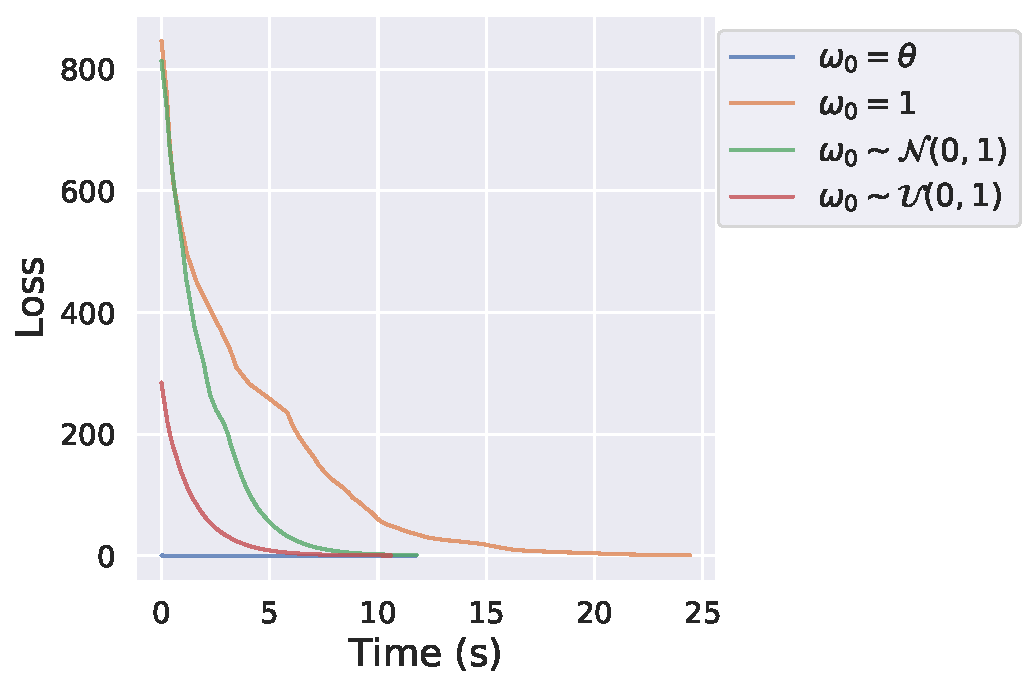
\includegraphics[width=0.7\textwidth]{./experiment2/w_0/sgd_loss_time.pdf}
		}
		\caption{}
		\label{eq:exp2_fig3}
	\end{figure}
	
	\begin{figure}[h]
		\centering{
		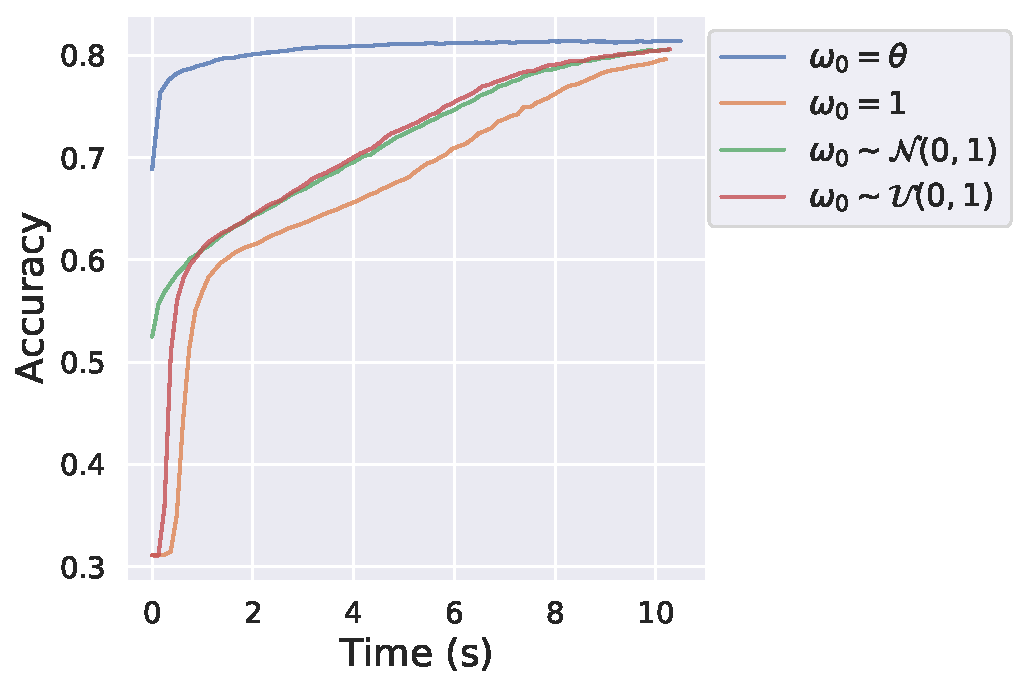
\includegraphics[width=0.7\textwidth]{./experiment2/w_0/sgd_acc_time.pdf}
		}
		\caption{}
		\label{eq:exp2_fig4}
	\end{figure}
	По-прежнему лучшим начальным приближением является $\omega_0=0$. Из необычного несложно заметить, что в отличие от эксперимента 1\footnote{В эксперименте 1 {\itshape accuracy} для $\omega_0 \neq 0$ равен $\approx 0.65$} в этом $accuracy$ для всех рассмотренных случаев значительно ближе к наилучшей оценке минимума для $\omega_0 = 0$ и достигается за меньшее количество времени чем для GD.

	\item {\bfseries  Выбор $batch\_size$}
	
	Фиксируем $\alpha = 0.1$, $\beta = 0.0347$, $\omega_0=0$ и рассмотрим различные параметры batch\_size (см. рис.\ref{eq:exp2_fig5}):
	\begin{figure*}[h]
        \begin{subfigure}{.5\textwidth}
            \centering
            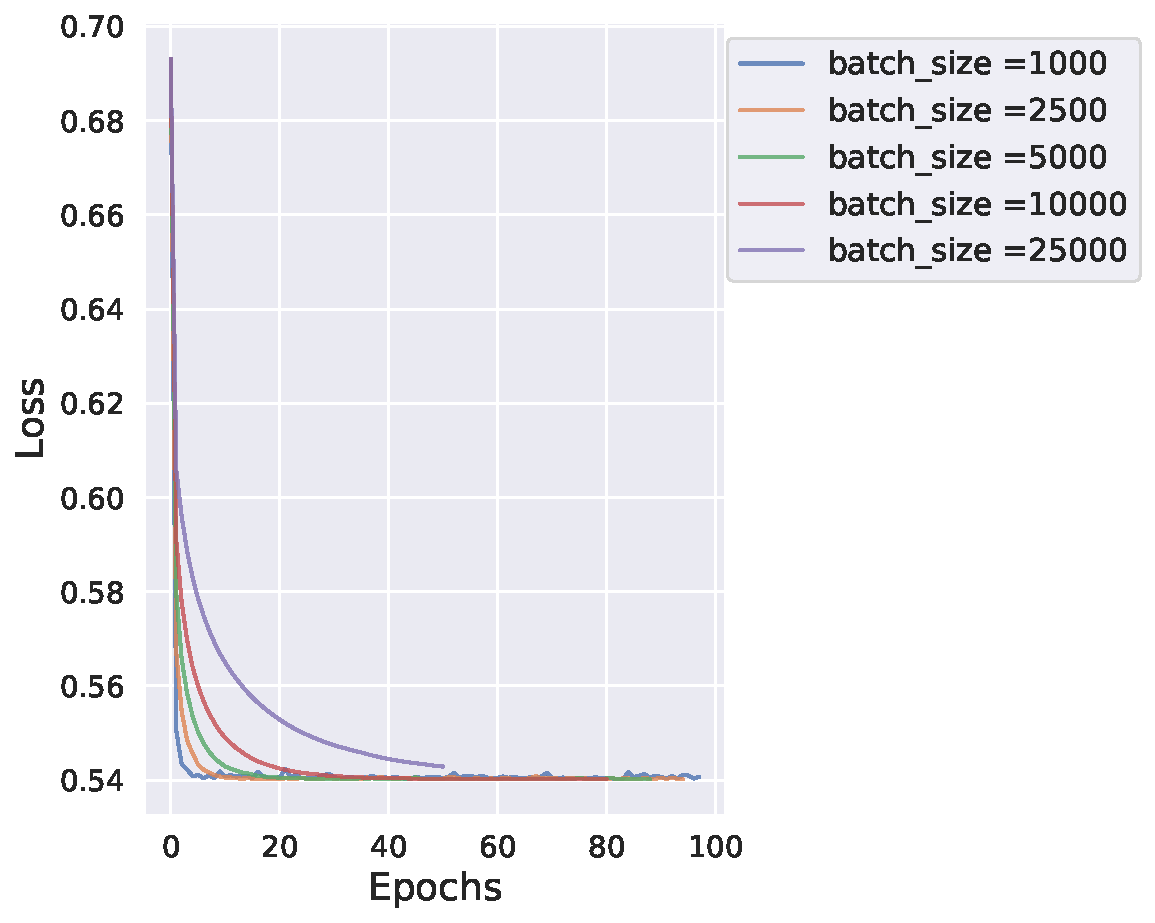
\includegraphics[width=\linewidth]{./experiment2/batch_size/sgd_loss_iters.pdf}
            \caption{}
        \end{subfigure}%
        \begin{subfigure}{.5\textwidth}
            \centering
            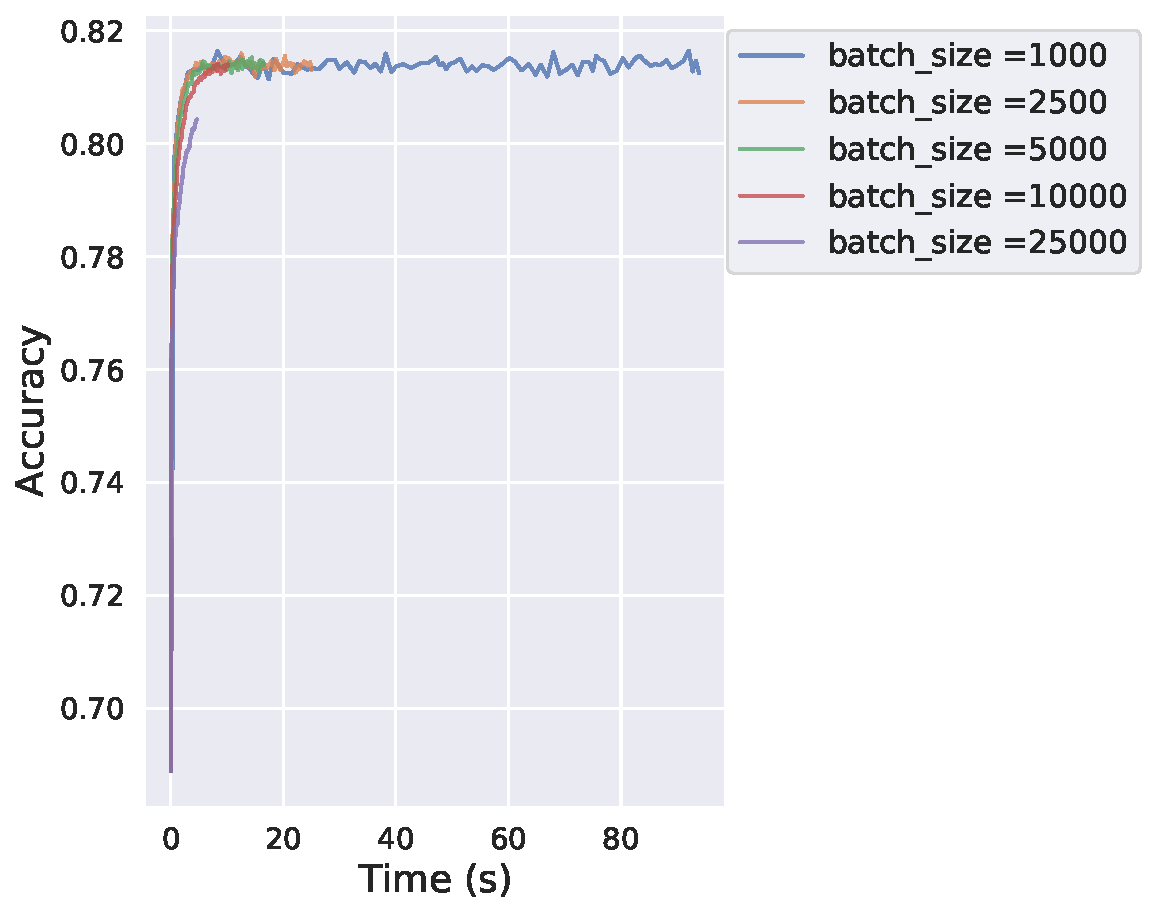
\includegraphics[width=\linewidth]{./experiment2/batch_size/sgd_acc_time.pdf}
            \caption{}
        \end{subfigure}
    \caption{}\label{eq:exp2_fig5}
    \end{figure*}
	Проанализировав рис.\ref{eq:exp2_fig5}, можно заметить что чем меньше размер батча тем меньше эпох, а значит, меньше потраченного времени нужно для достаточно неплохих оценок минимума функционала. Также видно, что с уменьшением батча увеличивается осцилляция. Хотя наилучшая точность на валидационной выборке была достигнута с $batch\_size = 1000$    ($accuracy = 0.8145$), в дальнейшем будет использоваться $batch\_size = 10000 $ ($accuracy = 0.8141$), поскольку он оптимален по нескольким параметрам: время (в $\approx\!8$  раз быстрее работает чем с $batch\_size = 1000$), $accuracy$ и устойчивость(меньше осцилляций, а значит при одних и тех же значениях метод будет получать более устойчивые оценки точности, чем с меньшими значениями размера)
\newpage
\subsubsection{Выводы эксперимента}
Для стохастического градиентного спуска оптимальным будет следующий выбор параметров:
\begin{itemize}
	\item $\alpha \lessapprox\!1.0$
	\item $\beta \lessapprox\!0.15$
	\item $w = 0$, $0 \in \mathbb{R}^D$
	\item $batch\_size \leq 10000$
\end{itemize}
\end{enumerate}
